\documentclass{article}

\usepackage[margin = 1in]{geometry}
\usepackage{graphicx}
\graphicspath{ {./images/} }

\title{Ch. 4 Solutions}
\author{Principles of Microeconomics}
\date{\today}

\begin{document}

\maketitle

\section*{Quick Quiz}

\begin{enumerate}

\item (c) -- A market doesn't have to be in a single location like options (a), (b), and (d).

\item (b) -- Sellers are price-takers in perfectly competitive markets.

\item (a) -- Eggs are mostly the same regardless of the seller, and there are too many buyers and sellers for any individual to affect the price. 

\item (b) -- A change in the price of hamburgers leads to a movement along the demand curve.

\item (a) -- When the price of a substitute goes up, the demand for pizza increases.

\item (d) -- Demand for an inferior good falls when incomes rise.

\item (a) -- movements along the supply curve come from changes in the price of the good.

\item (c) -- a decrease in the price of an input makes producing pizza more profitable, so supply shifts right.

\item (d) -- When the price of a substitute increases, demand increases.

\item (b) --
	\begin{center}
	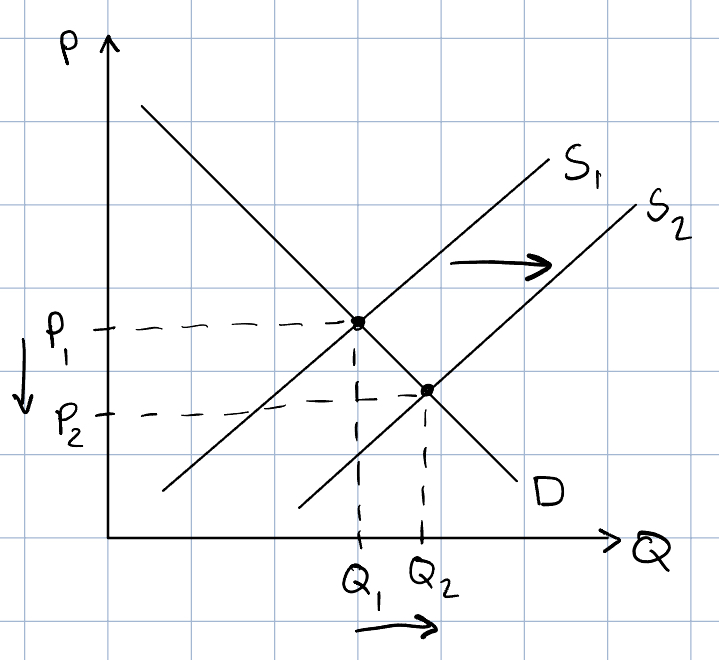
\includegraphics[width = 0.3\textwidth]{ch4_qq10}
	\end{center}

\item (a) --
	\begin{center}
	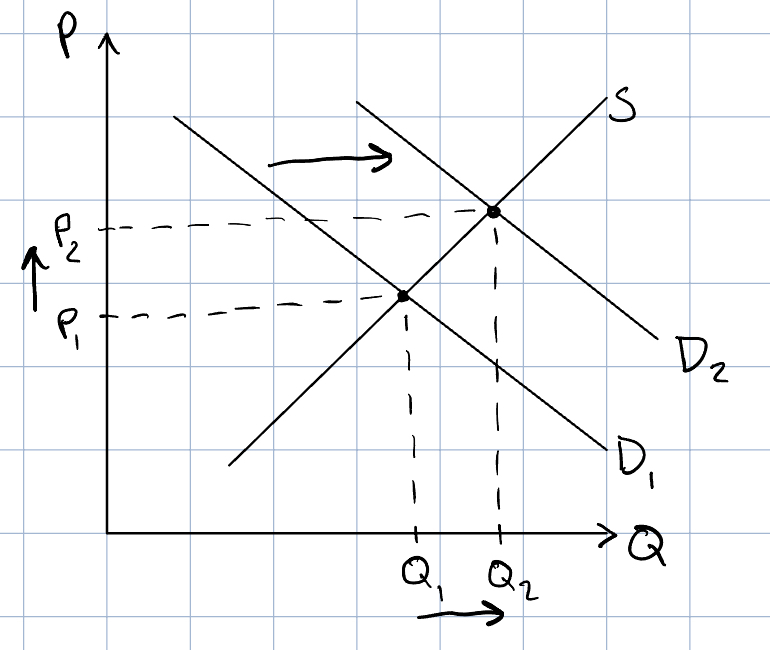
\includegraphics[width = 0.3\textwidth]{ch4_qq11}
	\end{center}

\item (c) -- For equilibrium price to increase and quantity to decrease, we need supply to shift left. That happens when input prices increase.
	\begin{center}
	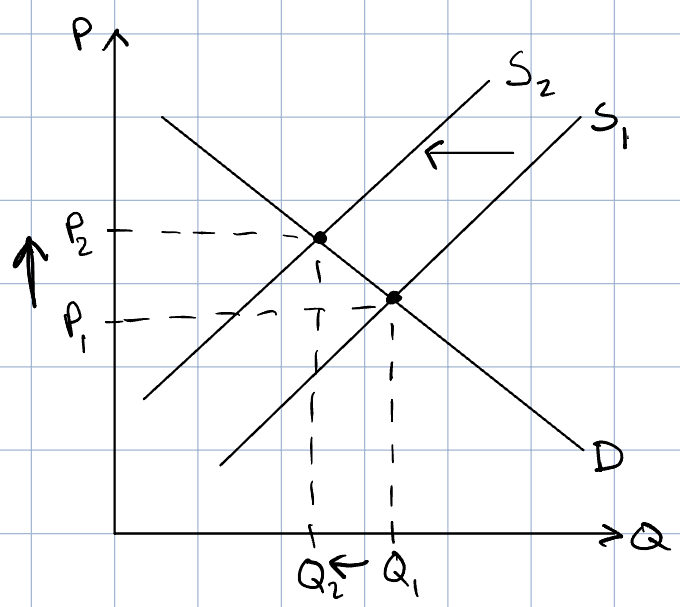
\includegraphics[width = 0.3\textwidth]{ch4_qq12}
	\end{center}
	
\item (d) -- If demand increases, that means the demand curve shifts right. As a result, the market moves to an equilibrium that's up and to the right on the supply curve. Since the equilibrium quantity increases, the quantity supplied increases as well.
	\begin{center}
	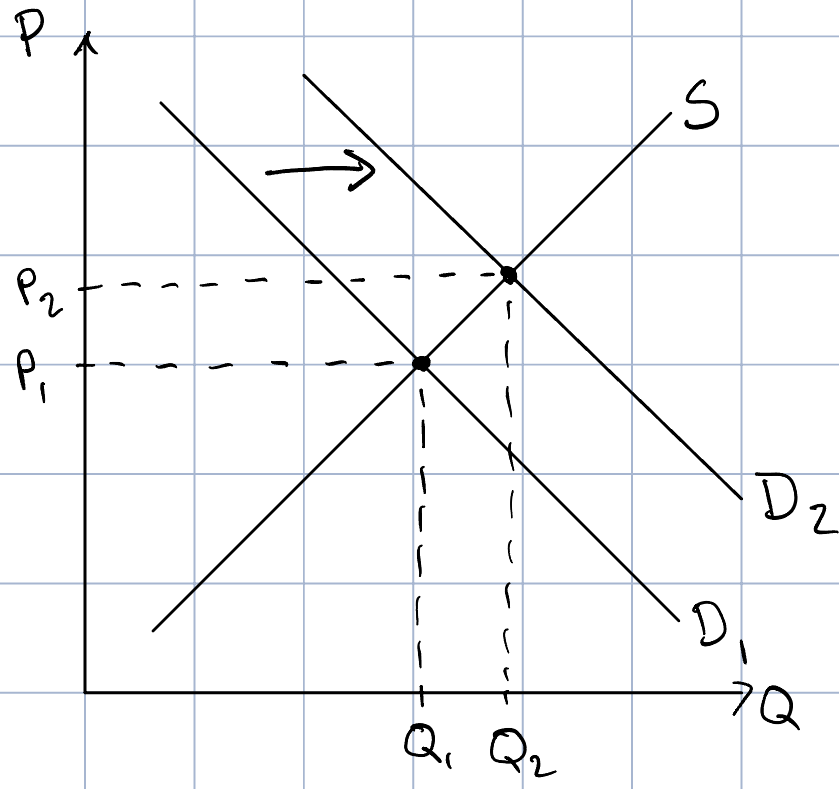
\includegraphics[width = 0.3\textwidth]{ch4_qq13}
	\end{center}

\end{enumerate}

\section*{Questions for Review}

\begin{enumerate}

\item A competitive market is a market in which there are so many buyers and sellers that no individual buyer or seller can significantly affect the price of the good. 

	A market that isn't perfectly competitive is a market with only one seller -- a monopoly.

\item A demand schedule is a table that lists the quantity demanded of a good at a variety of prices.

	A demand curve plots the relationship between the quantity demanded of a good and the price of that good.

	The two are related because a demand curve plots the points listed in a demand schedule.

	The demand curve slopes downward because consumers are willing and able to purchase less of a good as its price increases.

\setcounter{enumi}{2}

\item A change in tastes leads to a shift in the curve because a non-price determinant of quantity demanded is changing. 

	A change in price leads to a movement along the curve because the curve already shows how quantity demanded changes with price. 

\item Pumpkin juice is an inferior good because his demand for it rises as his income falls.

	His demand curve shifts right because he demands more. 

\item A supply schedule is a table that lists the quantity supplied of a good at a variety of prices.

	A supply curve is a plot of the relationship between the quantity supplied of a good and its price.
	
	The two are related because a supply curve plots the points listed in a supply schedule.
	
	The supply curve slopes upwards because producers are willing and able to sell more of a good as its price increases.
	
\item A change in producers' technology leads to a shift in the supply curve because a non-price determinant of quantity supplied is changing.

	A change in price leads to a movement along the supply curve because the curve already shows how quantity demanded changes with price.
	
\item The equilibrium of a market is the price and quantity at which quantity supplied equals quantity demanded. It's where the supply and demand curves intersect.

	If there's a shortage in the market, that means the market price is below the equilibrium price, and the quantity demanded is greater than the quantity supplied. When producers recognize the excess demand for their goods, they will raise their prices. That moves the economy from a shortage towards equilibrium.
	
	If there's a surplus in the market, that means the market price is above the equilibrium price, and the quantity demanded is less than the quantity supplied. When producers recognize that they can't sell all of their goods, they will cut their prices to attract buyers. That moves the economy from a surplus towards equilibrium.
	
\item When the price of beer rises, the supply of pizza stays the same, but the demand for pizza decreases. As a result, the quantity supplied and demanded decreases, and the price decreases as well.
	\begin{center}
	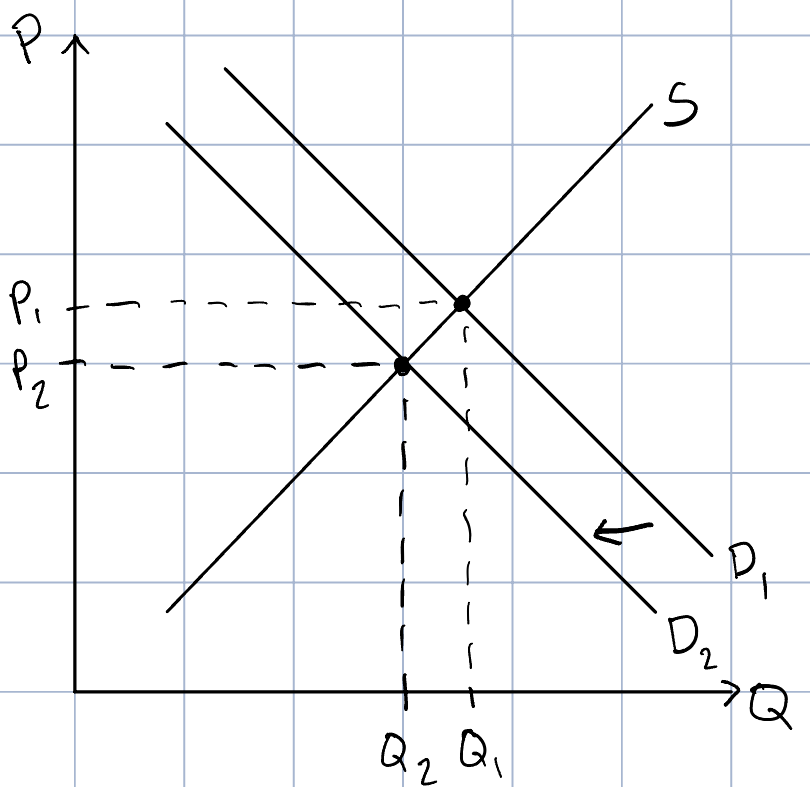
\includegraphics[width = 0.3\textwidth]{ch4_qfr8}
	\end{center}
	
\item Prices determine how much of a good consumers demand and how much producers supply. Prices move in a way that equalizes the quantity demanded and supplied. 

\end{enumerate}

\section*{Problems and Applications}

\begin{enumerate}

\item
	\begin{enumerate}
	
	\item The cold snap will increase the cost of oranges because orange farms will be less productive. Oranges are an input of orange juice, so the supply of OJ shifts to the left and increases the equilibrium price. 
	\begin{center}
	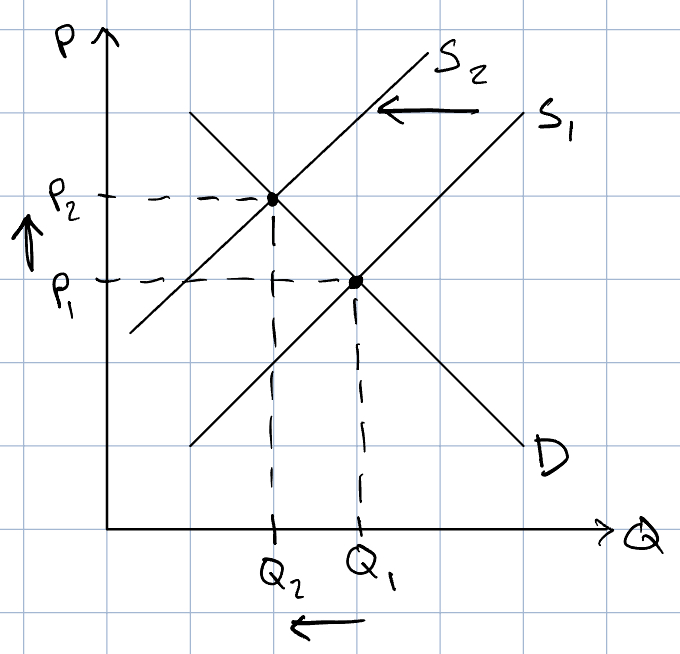
\includegraphics[width = 0.3\textwidth]{ch4_paa1a}
	\end{center}
	
	\item People's preferences for hotel rooms move away from the Caribbean and towards New England. That decreases demand and drives down the equilibrium price.
	\begin{center}
	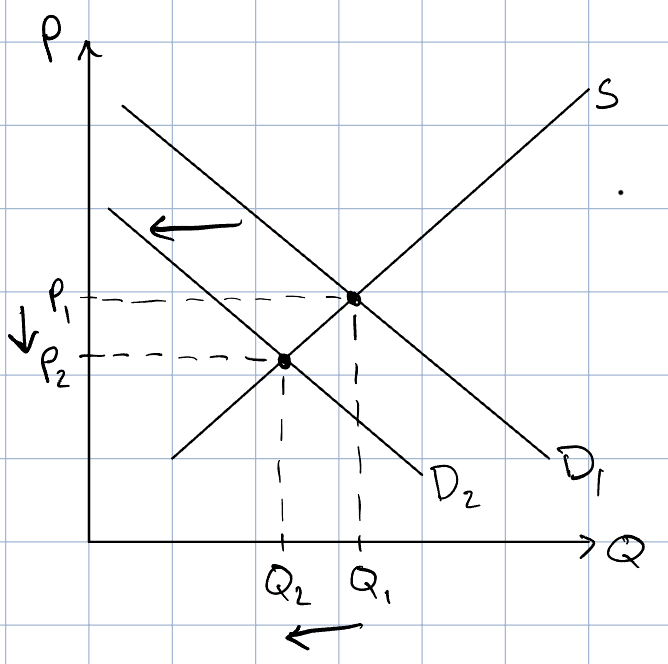
\includegraphics[width = 0.3\textwidth]{ch4_paa1b}
	\end{center}
	
	\item When war breaks out in the Middle East, it prevents many oil producers from selling their oil. That shifts the supply of gasoline left which in turn increases the price of gasoline. Gasoline and SUVs are complements, so when the price of gasoline goes up, demand for SUVs shifts left. As a result, the price of cars drops.
	\begin{center}
	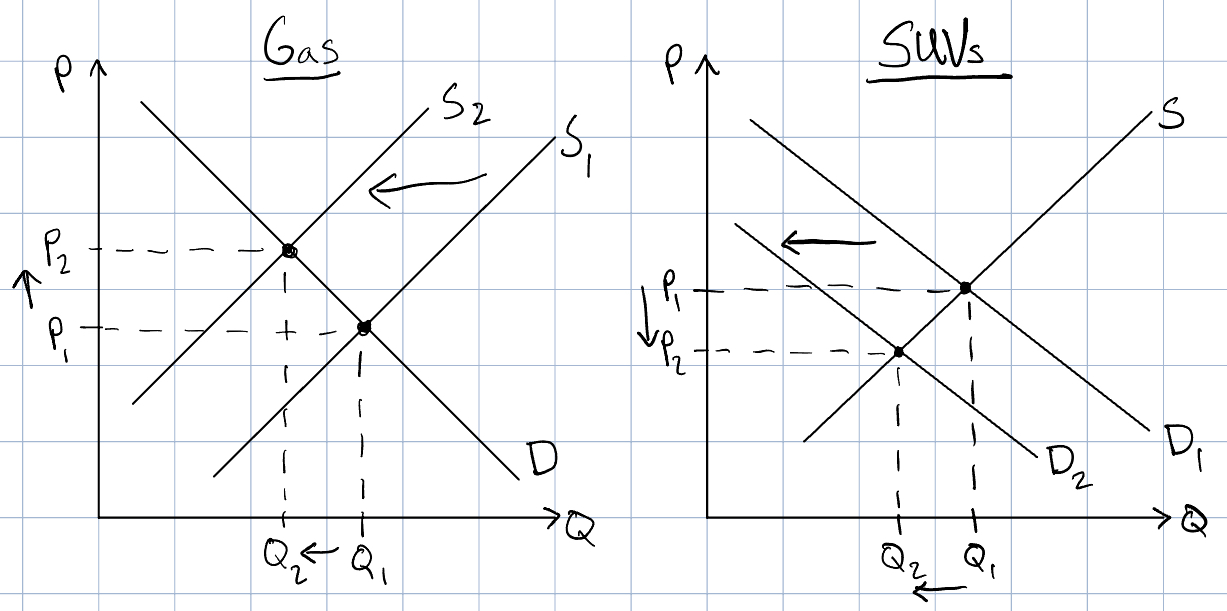
\includegraphics[width = 0.6\textwidth]{ch4_paa1c}
	\end{center}
	
	\end{enumerate}
	
\item False --An increase in the demand for notebooks is a rightward shift of the demand curve. When demand shifts right, the equilibrium quantity increases. That means quantity supplied and quantity demanded both increase.
 	\begin{center}
	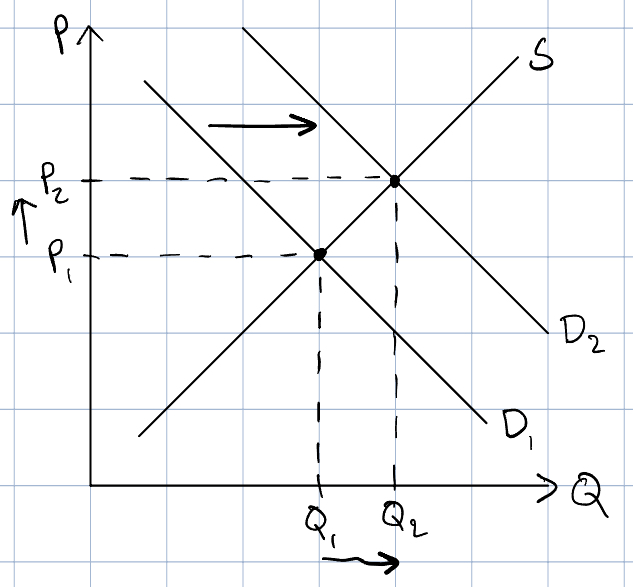
\includegraphics[width = 0.3\textwidth]{ch4_paa2}
	\end{center}
	
\item 
	\begin{enumerate}
	
	\item Having more children will increase people's taste for minivans and shift demand to the right. That increases the equilibrium price and quantity of minivans.
	\begin{center}
	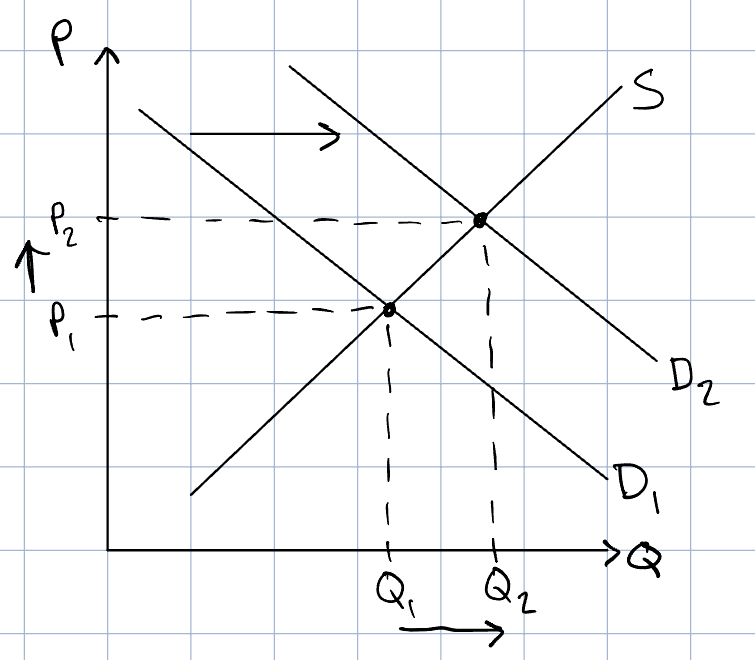
\includegraphics[width = 0.3\textwidth]{ch4_paa3a}
	\end{center}
	
	\item An input price has increased, so the supply of minivans will shift to the left. That increases equilibrium price and decreases equilibrium quantity.
	\begin{center}
	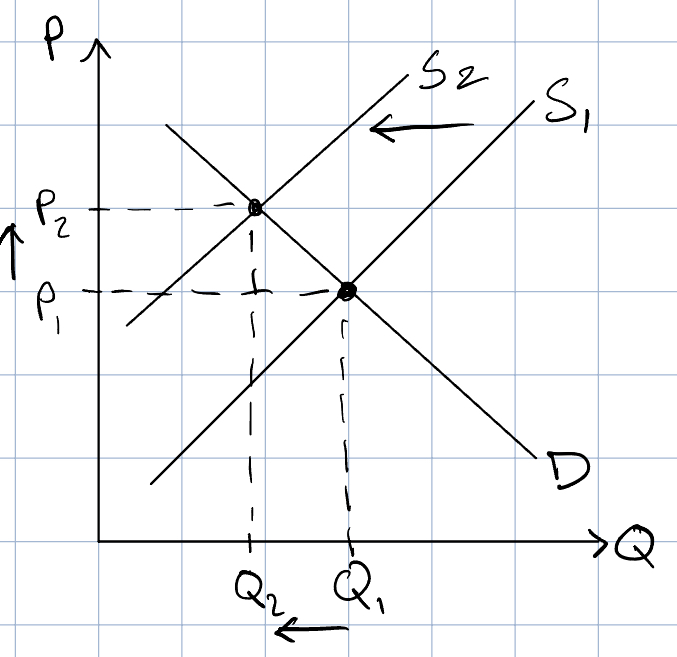
\includegraphics[width = 0.3\textwidth]{ch4_paa3b}
	\end{center}
	
	\item The advancement in production technology will shift supply to the right which lowers the equilibrium price and raises the equilibrium quantity.
	\begin{center}
	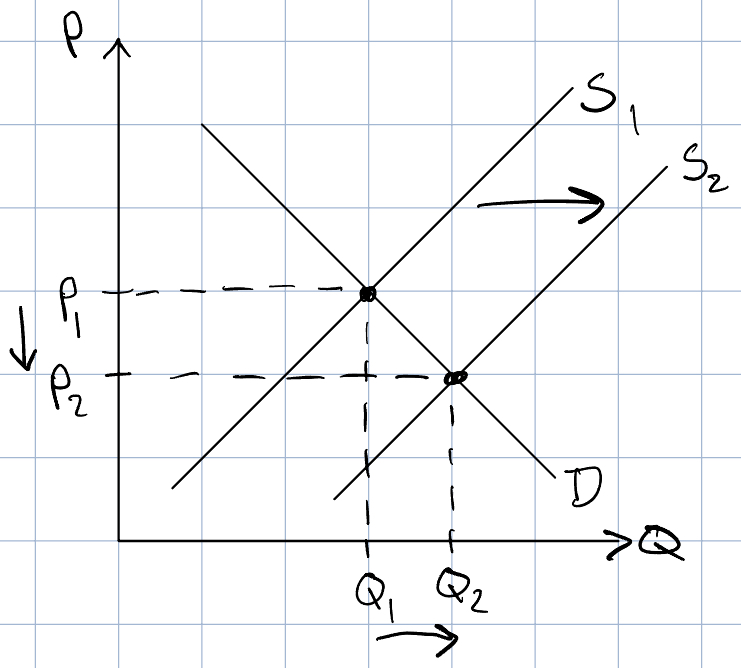
\includegraphics[width = 0.3\textwidth]{ch4_paa3c}
	\end{center}
	
	\item SUVs are a substitute for minivans, so when they get more expensive, demand for minivans increases. That increases the equilibrium price and quantity of minivans.
	\begin{center}
	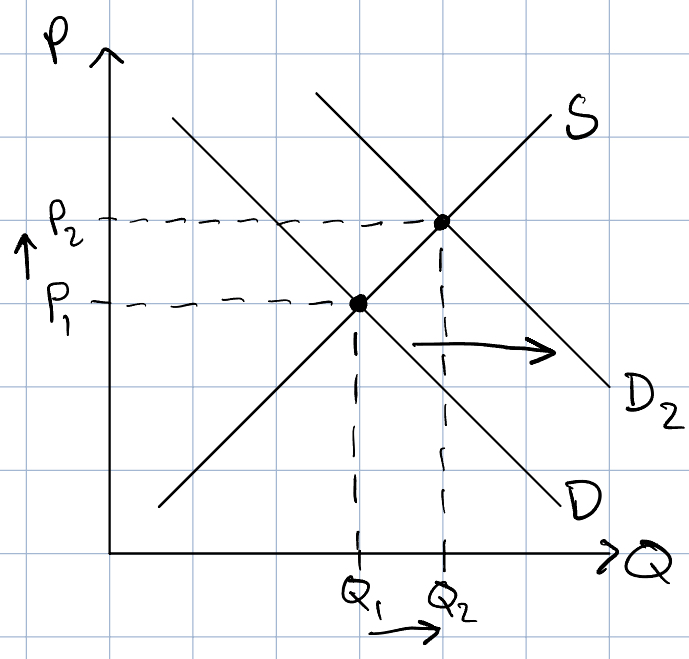
\includegraphics[width = 0.3\textwidth]{ch4_paa3d}
	\end{center}
		
	\item Minivans are normal goods, so when incomes decline, people buy fewer minivans. That shifts demand to the left which lowers the equilibrium price and quantity. 
	\begin{center}
	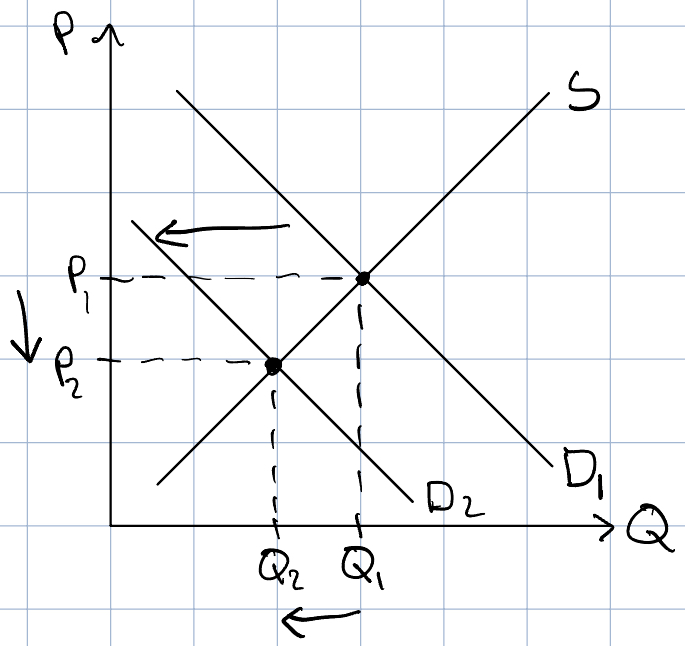
\includegraphics[width = 0.3\textwidth]{ch4_paa3e}
	\end{center}
	
	\end{enumerate}
	
\item
	\begin{enumerate}
	
	\item 
		
		\begin{itemize}
		
		\item Complements -- Video streaming and TV screens are typically consumed together. 
		
		\item Substitutes -- Video streaming and movie tickets are typically consumed in place of each other. 
		
		\item Substitutes -- TV screens and movie tickets are typically consumed in place of each other. 
		
		\end{itemize}
		
	\item The lower cost of manufacturing will shift the supply curve for TV screens to the right which decreases equilibrium price and increases equilibrium quantity.
	\begin{center}
	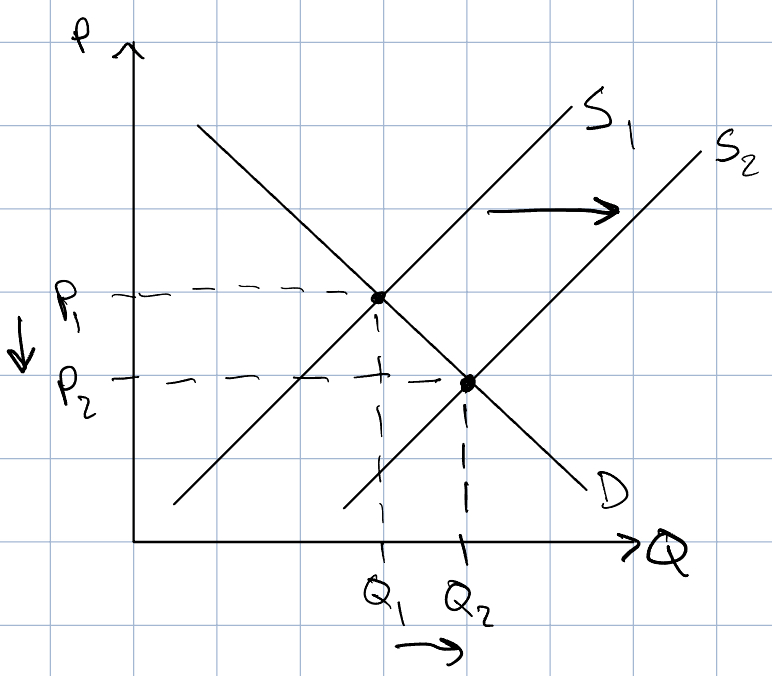
\includegraphics[width = 0.3\textwidth]{ch4_paa4b}
	\end{center}
	
	\item Video streaming and TV screens are complements, so when the price of TV screens goes down, demand for streaming shifts right. As a result, price increases, and quantity increases.
	\begin{center}
	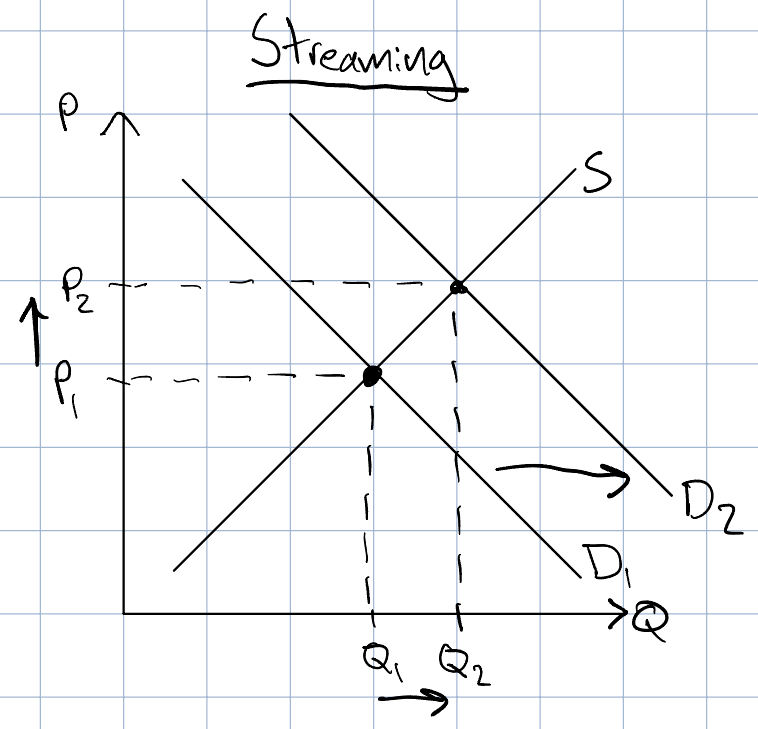
\includegraphics[width = 0.3\textwidth]{ch4_paa4c_streaming}
	\end{center}
	
	Movie tickets and TV screens are substitutes, so when the price of TV screens goes down, demand for movie tickets shifts left. As a result, price decreases, and quantity decreases.
	\begin{center}
	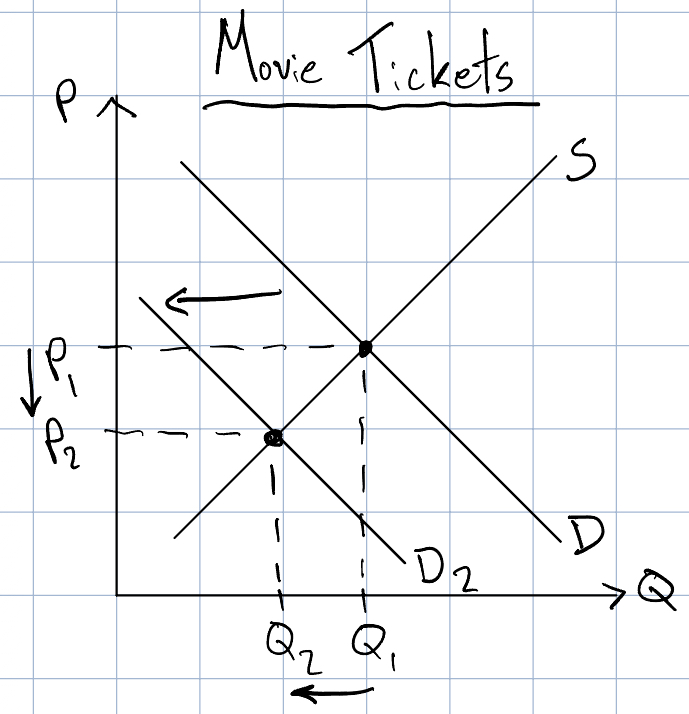
\includegraphics[width = 0.3\textwidth]{ch4_paa4c_tix}
	\end{center}
	
	\end{enumerate}
	
\item Computer chips are an input for computers, so when the price of computer chips goes down, the supply of computers increases. As a result, price decreases and quantity increases in the market for computers.
	\begin{center}
	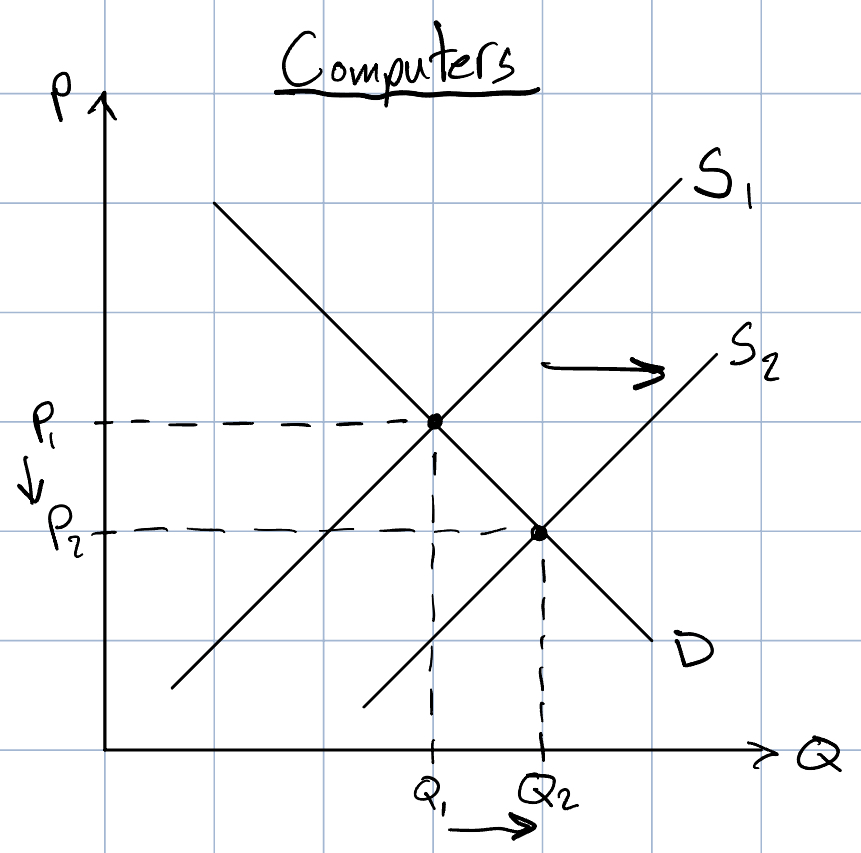
\includegraphics[width = 0.3\textwidth]{ch4_paa5_computers}
	\end{center} 
	
	Computers and computer software are complements, so when the price of computers decreases, demand for computer software increases. That increases the price and quantity of computer software.
	\begin{center}
	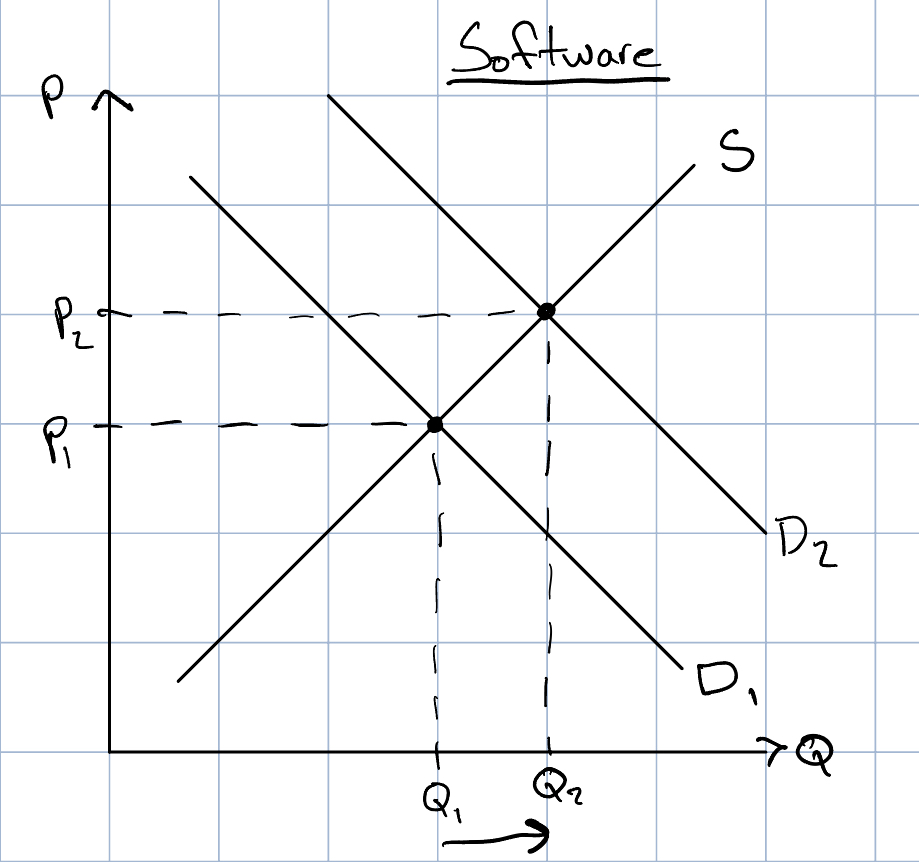
\includegraphics[width = 0.3\textwidth]{ch4_paa5_software}
	\end{center}
	
	Computers and typewriters are substitutes, so when the price of computers decreases, demand for typewriters decreases. That decreases the price and quantity of typewriters. 
	\begin{center}
	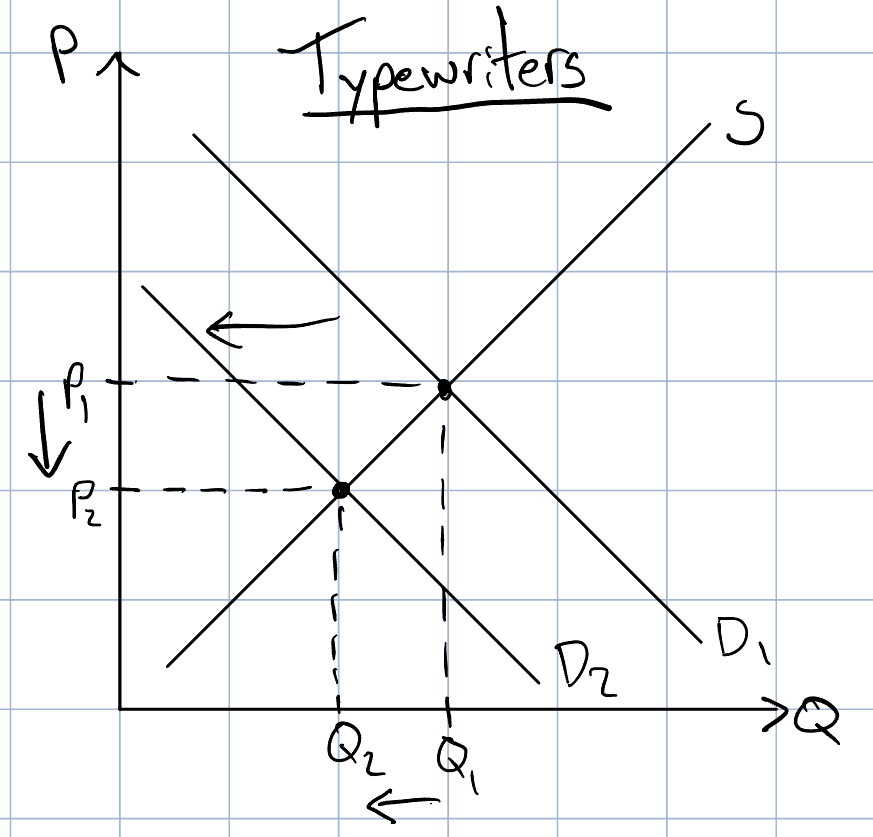
\includegraphics[width = 0.3\textwidth]{ch4_paa5_typewriters}
	\end{center}
	
\item
	\begin{enumerate}
	
	\item The damaged crop will increase the price of cotton, so an input for sweatshirts becomes more expensive. That shifts supply left which increases equilibrium price and decreases equilibrium quantity.
	\begin{center}
	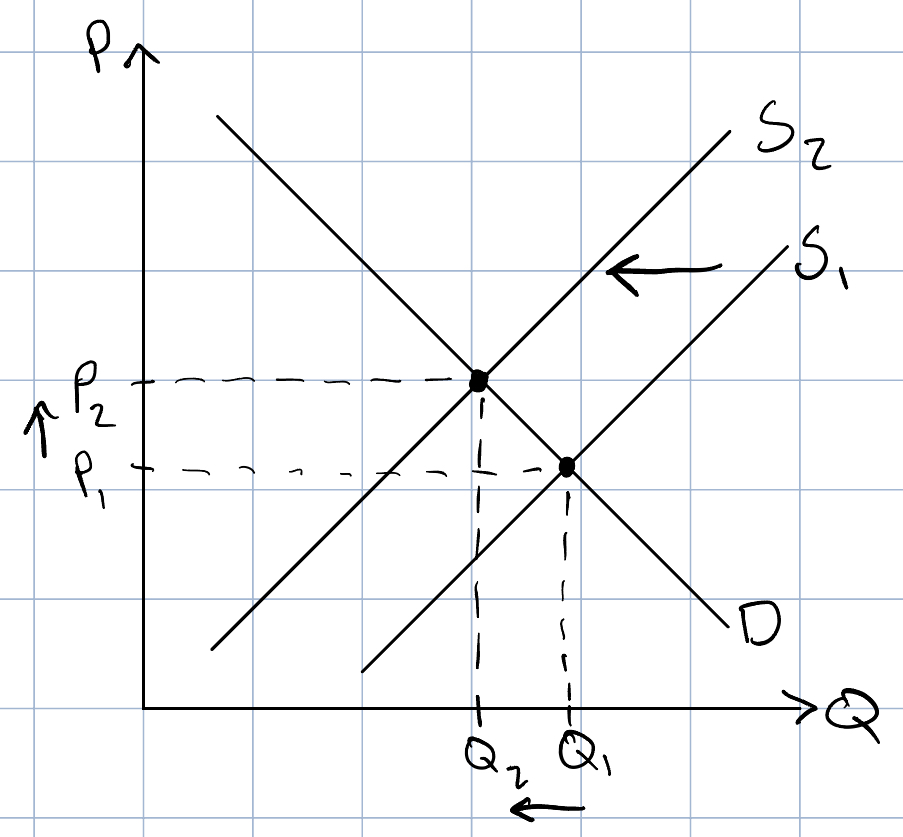
\includegraphics[width = 0.3\textwidth]{ch4_paa6a}
	\end{center}
	
	\item The price of a substitute decreases, so demand shifts left. That decreases equilibrium price and quantity.
	\begin{center}
	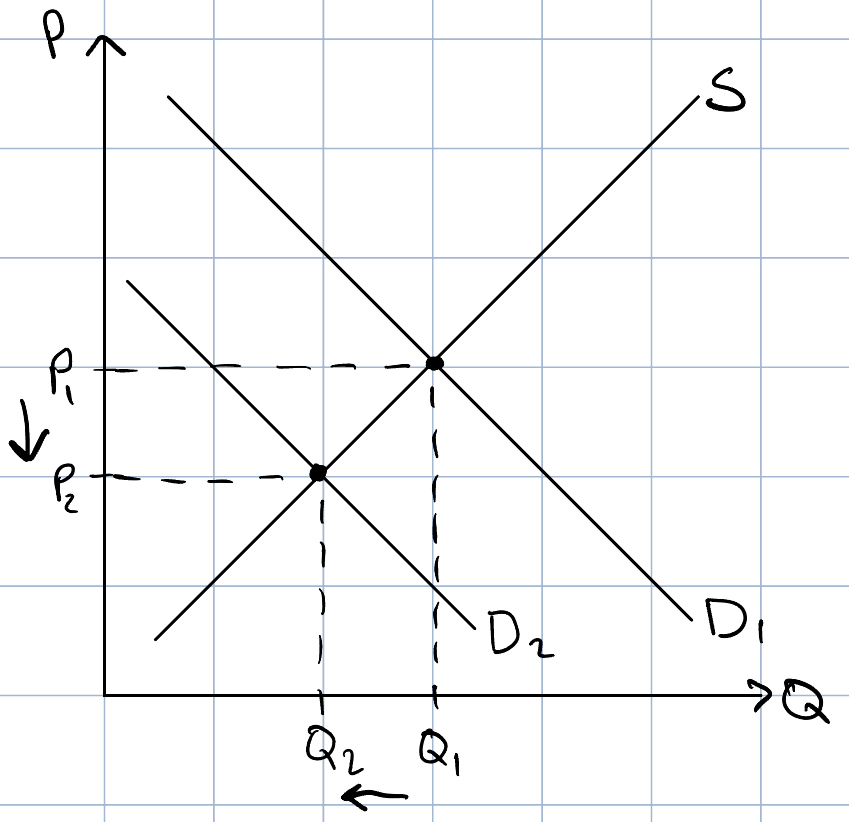
\includegraphics[width = 0.3\textwidth]{ch4_paa6b}
	\end{center}
	
	\item The college mandate will increase the number of buyers which will shift demand right. That increases equilibrium quantity and price.
	\begin{center}
	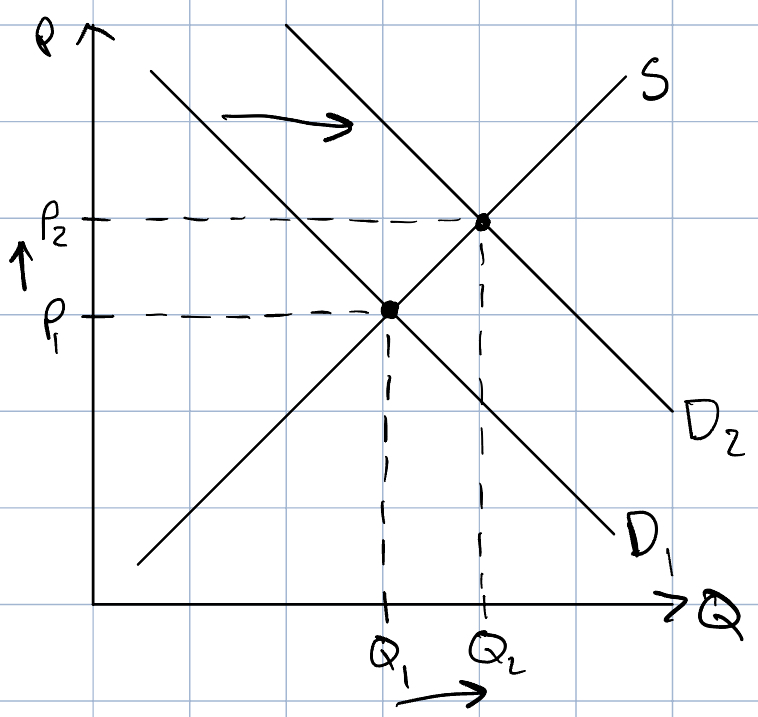
\includegraphics[width = 0.3\textwidth]{ch4_paa6c}
	\end{center}
	
	\item The improvement in production technology will increase supply. That increases equilibrium quantity and decreases equilibrium price.
	\begin{center}
	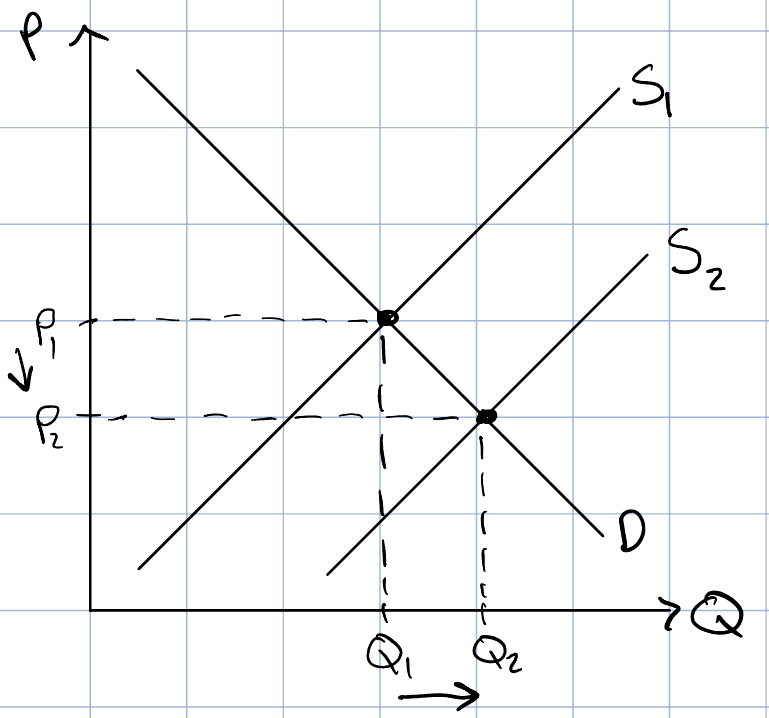
\includegraphics[width = 0.3\textwidth]{ch4_paa6d}
	\end{center}
	
	\end{enumerate}
	
\item If the price of hot dogs rises, demand for its complement, ketchup, will shift left. As a result, the price and quantity of ketchup will decrease.
	\begin{center}
	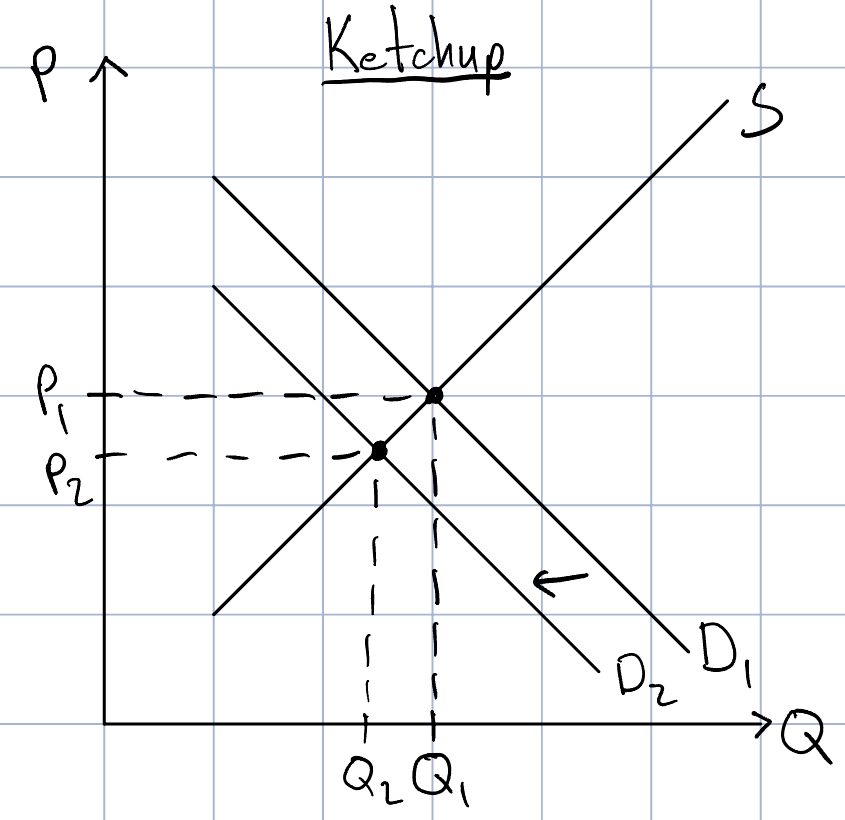
\includegraphics[width = 0.3\textwidth]{ch4_paa7_ketchup}
	\end{center}
	Tomatoes are an input of ketchup. Therefore, if the quantity of ketchup decreases, producers of ketchup will demand fewer tomatoes. As a result, demand for tomatoes will shift left, and the price and quantity of tomatoes will decrease.
	\begin{center}
	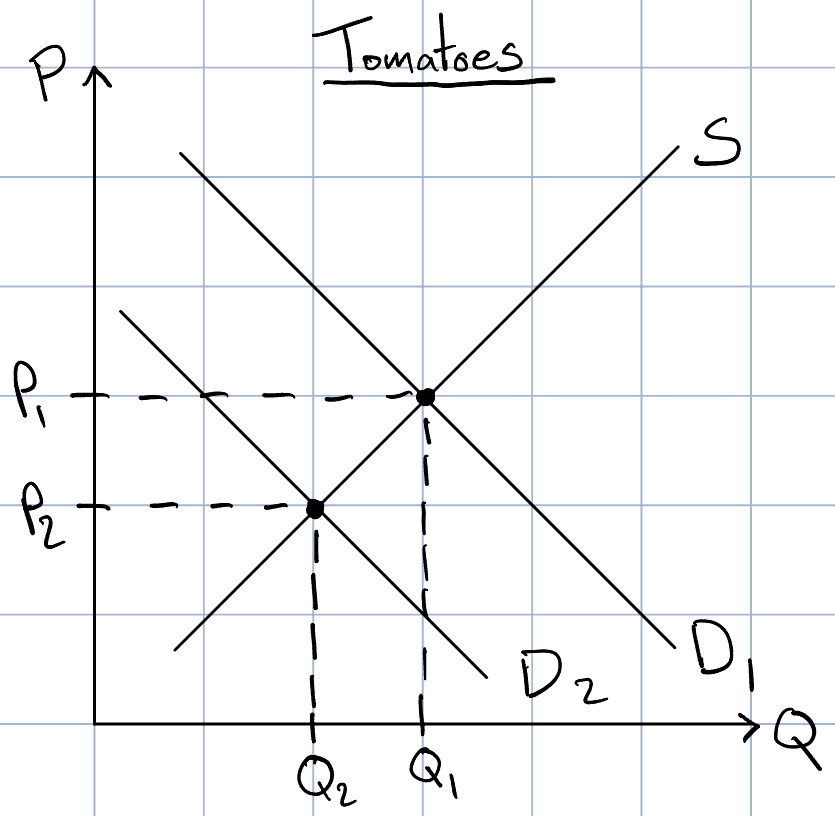
\includegraphics[width = 0.3\textwidth]{ch4_paa7_tomatoes}
	\end{center}
	Tomatoes are also an input of tomato juice. If the price of tomatoes decreases, the supply of tomato juice will shift to the right. As a result, the price of tomato juice will decrease, and the quantity of tomato juice will increase.
	\begin{center}
	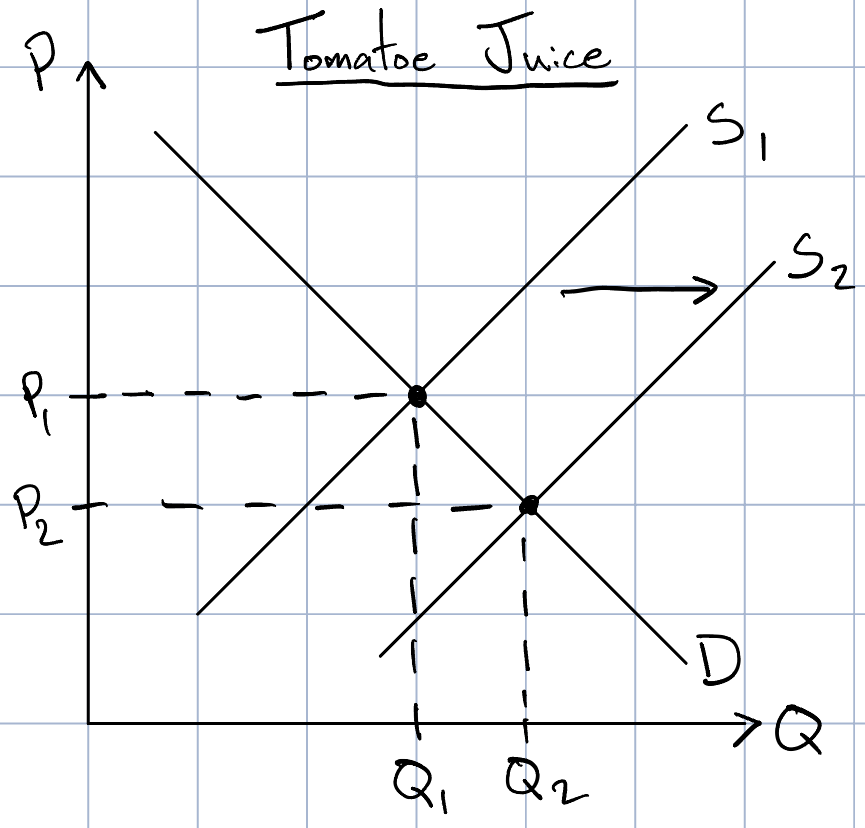
\includegraphics[width = 0.3\textwidth]{ch4_paa7_tomato_juice}
	\end{center}
	Tomato juice is a substitute for orange juice. If the price of tomato juice decreases, demand for orange juice will shift left. As a result, the price and quantity of orange juice will decrease.
	\begin{center}
	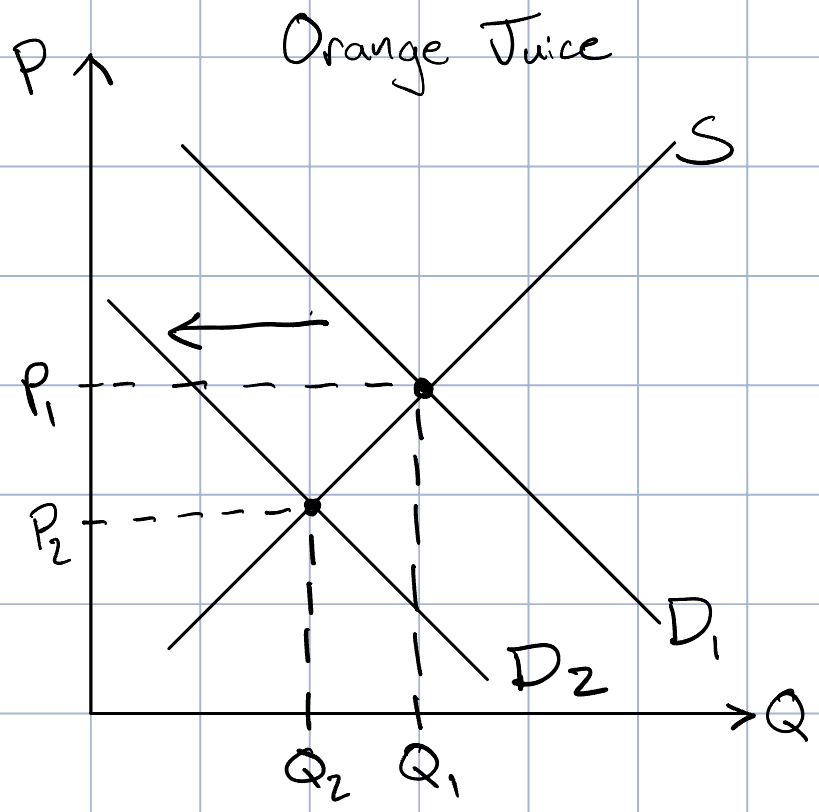
\includegraphics[width = 0.3\textwidth]{ch4_paa7_oj}
	\end{center}
	
\item
	\begin{enumerate}
	
	\item The equilibrium price is \$6 because that's the price at which $Q_S = Q_D$. The equilibrium quantity is 81.
		\begin{center}
		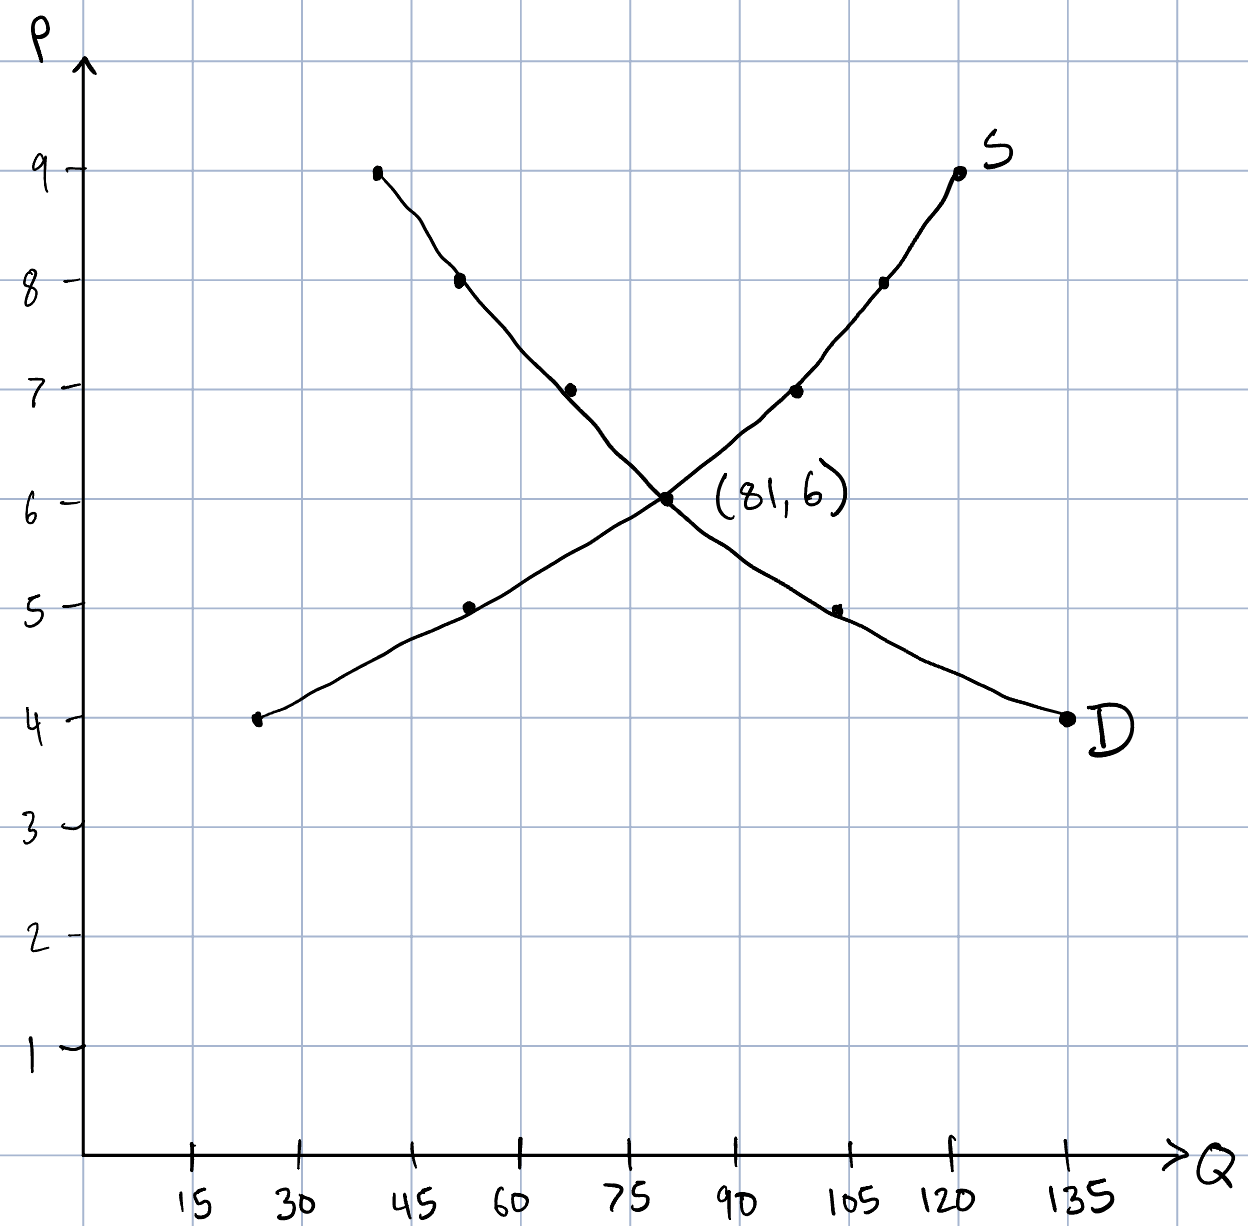
\includegraphics[width = 0.5\textwidth]{ch4_paa8a}
		\end{center}
		
	\item There would be a surplus in which case $Q_S > Q_D$. Producers wouldn't be able to sell all of their goods, so they would start cutting their prices to attract more buyers. That would decrease the quantity supplied and increase the quantity demanded, so it would move the market towards equilibrium.
	
	\item There would be a shortage in which case $Q_S < Q_D$. Producers would recognize the excess demand for their goods, so they would start to increase their prices. That would increase the quantity supplied and decrease the quantity demanded, so it would move the market towards equilibrium.
	
	\end{enumerate}

\end{enumerate}

\end{document}